\chapter{}
\section{RCL}

\noindent En el curso se trabajara con circuitos electriocos RCL en serie. El objetivo de estos problemas que calcular la
corriente I que circula por todo el circuito. Teniendo en cuenta que  $ I = \frac{dQ}{dt} $, donde Q es la carga.
\bigskip

\dfn{La ecuacion de un circuito RCL}{
    $$ L\frac{d^2Q}{dt^2} + R \frac{dQ}{dt} + \frac{1}{C}Q = V(t)$$
    Donde:
    \begin{itemize}
        \item L es la inductancia, se mide en Henrys (H)
        \item R es la resistencia, se mide en Ohms ($\Omega$)
        \item C es la capacitancia, se mide en Farads (F)
        \item V(t) es la fuente de voltaje, se mide en Volts (V)
        \item Q(t) es la carga, se mide en Coulombs (C)
        \item I(t) es la corriente, se mide en Amperes (A)
    \end{itemize}
}

Los problemas pueden ser resueltos por diversos metodos dependiendo de la configuración de componentes, desde metodo 
de factor integrante hasta MVP.


\subsection{Ejercicios}
    \qs{}{ En un circuito RC en serie se tiene una fuente constante de 50 V , además
        R = 100Ω y C = 5 x $10^{-3}$ F . Si inicialmente el condensador está descargado
        ¿Cuánto tiempo tarda aproximadamente en cargarse?}

    \sol
    \newline
    Como no hay inductancia, la ecuación queda:
    $$ R\frac{dQ}{dt} + \frac{1}{C}Q = V(t) $$

    Reemplazando valores:

    $$ 100\frac{dQ}{dt} + \frac{1}{5 x 10^{-3}}Q = 50 $$
    $$ 100\frac{dQ}{dt} + 200Q = 50 $$
    $$ \frac{dQ}{dt} + 2Q  = \frac{1}{2} $$

    Con la ecuacion diferencial obtenida es posible empezar a resolverla usando el metodo de factor integrante:

    $$ \mu = e^{\int 2 dt} = e^{2t} $$

    Aplicar la forma del factor integrante ($ y = \frac{1}{\mu} \int{(\mu)(Q(x))}dx  $)

    $$ \frac{1}{e^{2t}} \int{(e^{2t})(50)}dt  = Q$$
    $$ \frac{50}{e^{2t}} \int(e^{2t}) dt = Q$$
    $$ \frac{50}{e^{2t}} (\frac{e^{2t}}{200} + C) = Q$$
    $$ \frac{1}{4} + Ce^{-2t} = Q$$


    Como el condesador esta descargado, no hay carga presente eal inicio, es por ello que se puede obtener la constante C en
    $t_0$:

    Si $Q(0) = 0$, entonces :
    $$ \frac{1}{4} + Ce^{-2(0)} = 0 $$
    $$ \frac{1}{4} + C = 0 $$
    $$ C = -\frac{1}{4} $$


    Por lo tanto la ecuacion queda:
    $$ Q = \frac{1}{4} - \frac{1}{4}e^{-2t} $$

    Con la funcion obtenida podemos calcular el tiempo que tarda en cargarse el condensador. Pero como la funcion 
    posee una asintota vertical para $Q = \frac{1}{4}$, se puede decir que el condensador nunca se cargara completamente, pero
    se puede asumir que una carga completa es aproximadamente el $99.9\%$ de la carga maxima.
    
    $$ Q(t) = \frac{1}{4} - \frac{1}{4}e^{-2t} = \frac{1}{4} * 99.9\% $$
    $$ \frac{1}{4}e^{-2t} = \frac{1}{4} * 0.001 $$
    $$ e^{-2t} = 0.001 $$
    $$ -2t = ln(0.001) $$
    $$ t = 3.4538$$

    %%%%%%%%%%%%%%%%%%%%%%%%%%%%%%%%%%%%%%%%%%%%%%%%%%%%%%%%%%%%%%%%
    \qs{}{ En el circuito de la figura suponga que L = 5H, R = 25 $\Omega$, y la fuente E es una batería que suministra 
    un voltaje constante de 100V.El interruptor se encuentra en la posición 1 por un largo tiuempo de tal manera que fluye
    una corriente estacionaria de 4A. En el tiempo t = 0s el interruptor se mueve a la posición 2. Determine la corriente}

    \begin{center}
        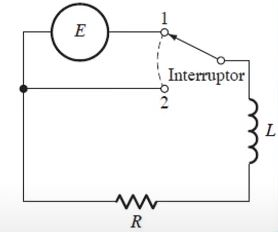
\includegraphics[scale=1]{chapters/4/images/ej3.jpg}   
    \end{center}

    \sol
    \newline
    Tenemos los siguientes datos:
    \begin{itemize}
        \item L = 5H
        \item R = 25 $\Omega$
        \item $V(t)$ = 0V
        \item $I(0)$ = 4A
    \end{itemize}

    Como el tiempo empieza recien cuando se pone el interrumptor en la posición 2, el votaje es 0V, por lo tanto la 
    ecuacion quedaria de la siguiente manera:

    $$ 5\frac{d^2Q}{dt^2} + 25\frac{dQ}{dt} = 0$$

    Para hallar la funcion de la corriente, se puede reemplazar $I = \frac{dQ}{dt}$, por lo tanto la ecuacion queda:

    $$ 5\frac{dI}{dt} + 25I = 0$$

    Se puede resolver por el metodo de separación de variables:

    $$ \frac{dI}{dt} + 5I = 0 $$
    $$ \frac{dI}{dt} = -5I $$
    $$ \frac{1}{I}dI = -5dt $$
    
    Integrando:
    $$ \int{\frac{1}{I}dI} = \int{-5dt} $$
    $$ ln(|I|) = -5t + C $$
    $$ |I| = e^{-5t + C} $$
    
    La solucion planteada es:
    $$ I = e^{-5t}e^{C} $$
    $$ I = Ce^{-5t} $$

    Reemplazando en $$ t = 0 $$:
    $$ 4 = Ce^{-5(0)} $$
    $$ 4 = C $$

    La funcion final es:
    $$ I = 4e^{-5t} $$

    %%%%%%%%%%%%%%%%%%%%%%%%%%%%%%%%%%%%%%%%%%%%%%%%%%%%%%%%%%%%%%%%
